\chapter{Introduction}

\epigraph{Learning to read is probably the most difficult and revolutionary thing that happens to the human brain, and if you don't believe that, watch an illiterate adult try to do it.}{John Steinbeck}

\section{Cognitive flexibility and network architecture}

The human brain is remarkable for its flexibility: a person can interpret physical sensations, coordinate complex movements, interpret subtle social cues, construct meaning from sounds, embolden a person with courage or freeze them with embarassment. And people perform all of these incredible calculations at the same time, without becoming confused or consternated. This arsenal of skills, which is rivaled by few if any other species in the animal kingdom, can only be possible through an efficient neural infrastructure. Neural areas responsible for snesory processing, executive decision-making, top-down attention and intrinsic motivation must all be able to interact quickly to react to changing environmental demands. 

The organizing structures and mechanisms that facilitate the brain's activity are collectively referred to as its \textit{network architecture}. The brain's network architecture has been studied on many scales -- from molecules and synapses to brain systems -- and with many techniques -- from electron microscopy to electroencephalography. More recently, advances in magnetic resonance imaging (MRI) have allowed researchers to investigate the brain's structural connectivity as well as its more fluid functional connectivity \citep{Betzel2013}. These two domains of inquiry can be thought of as the patterns of wiring and engagement between large patches of cortex, respectively. While our understanding of these patterns is becoming increasingly refined, there remain important questions, especially around the extent to which differences in network architecture are responsible for differences in individual behavior and development \citep{Petersen2015}.

\begin{figure}[t]
	\centering
	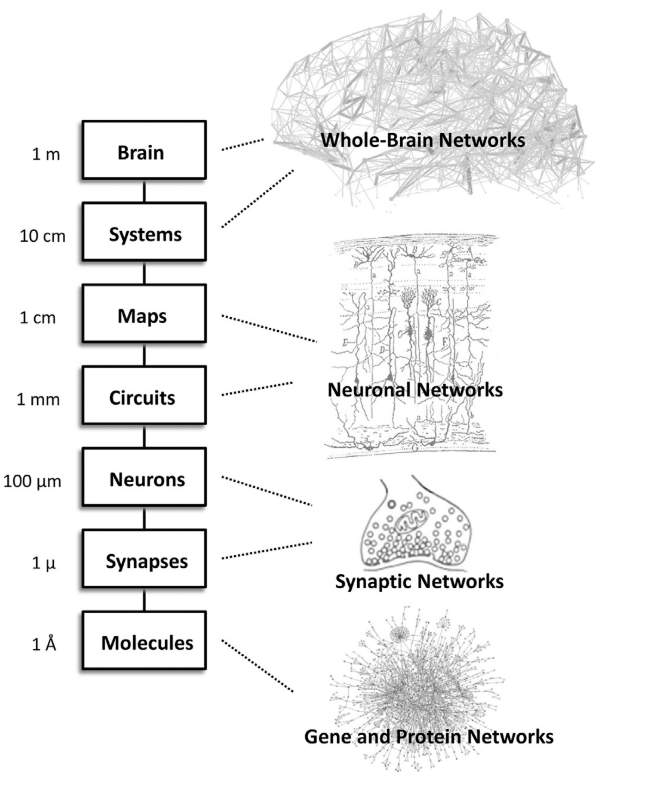
\includegraphics[height=4in]{ch6-multi-scale-connectivity-analysis}
	\caption[Network architecture at multiple scales.]{Network architecture at multiple scales of inquiry. The brain is organized in a manner that optimizes the trade-off between connectedness and metabolic efficiency. This results in small-world properties, including modularity, at multiple scales. In this dissertation, we focus on these properties in whole-brain networks. Figure from \citep{Petersen2015}.}
	\label{fig:ch6-multi-scale-connectivity-analysis}
\end{figure}

One of the challenges is that the methods and body of knowledge about large-scale network architecture have only recently begun to reach a consensus about fundamental points. This stands in contrast to the work mapping cognitive skills to specific parts of the brain conducted by the neuroscience community for the past several decades \citep{Yarkoni2011}. To understand how individual variability in brain structure and function drive individual differences in behavior and cognition, it will be critical to go creating ``population averages'' of brain networks, and to bridge the extant and mature literature on brain activity elicited by specific cognitive processes with the nascent literature on anatomical and functional networks of individuals. This will give provide a more holistic perspective on the neurobiological mechanisms, including the relationship between local processing and integration between separate cognitive systems. 

Comparing findings between the two approaches with a well-understood model system can be a powerful way to synthesize findings. The act of reading is a potent candidate: reading requires the tuning of specific and localized neuronal systems such as the visual word form area \citep{McCandliss2003}, as well as global systems that integrate information across sensory, associative and motor systems \citep{Price2012}. It is a learned skill, as well, so the effects of education and development are ripe for study \citep{Saygin2016}, and there are many detailed methods for comparing individual differences in reading expertise \citep{Woodcock1998}. 

In this dissertation, we flesh out a description of the network-level processes important for reading comprehension, how they form a basis for individual differences, and how aspects of functional network architecture change throughout the lifespan. This chapter lays the theoretical groundwork. First, we describe reading and our rationale for selecting it as a candidate cognitive process. we then describe metrics for measuring different aspects of network architecture and their potential significance to cognitive models. Next, we connect principal aspects of a network persepctive (especially RSNs and hubs) to reading processes and dyslexia. Finally, I discuss how maturation and education throughout development influence both reading skill and network architecture, and how the two might interact. I will then outline the four studies undertaken to establish the importance of this network approach to reading comprehension, and more broadly, cognitive flexibility.

\section{Reading is a whole-brain activity}

Reading is a complex cognitive act. To read, individuals must precisely control visual attention, map symbols to sounds, extract meaning from words, maintain and update a mental model of the text events, inhibit unimportant associations, and make appropriate inferences. Consequently, reading difficulty can arise from many sources \citep{Pennington2009, vanderLely2010}. To further complicate matters, people who struggle with reading also commonly struggle with other learning and developmental disorders, such as specific language impairment and attention deficit / hyperactivity disorder \citep{Pennington2006, Margari2013}.

Despite these complexities, the most common aim of reading instruction and intervention is to build fast and efficient orthographic-phonological mapping. That is because teaching these skills is concrete and effective \citep{NationalReadingPanel2000}. Decoding is also a bottleneck to semantic processes: if an individual cannot decipher individual words, they will not be able to understand blocks of text. However, there are many individuals who struggle primarily with reading comprehension, but understanding the specific causes of their struggle is difficult \citep{Cain2006}. One issue is that the component skills in comprehension are less mechanical and accessible than those for word reading. For example, although vocabulary size is often used as a proxy for the ability to comprehend speech \citep{Spencer2014}, it does not account for important executive and attention skills. Passage comprehension measures, on the other hand, are highly variable in their administration, skills assessed and resulting measures \citep{Cutting2009a}.

Neuroimaging provides an alternative way of assessing what makes good readers successful, and its use has yielded valuable insights into the neural mechanisms of typical and atypical reading. Researchers have shown that reading co-opts the brain's visual system to introduce a new input pathway into existing language comprehension circuitry \citep{Jobard2007}. As text complexity increases, a larger demand is made on support systems, and activation becomes more bilateral and widespread \citep{Xu2005}.  Meta-analyses show that individuals with reading difficulty typically exhibit underactivation in areas responsible for recognizing symbol units, parsing acoustic sounds into phonological units, and binding letters to sounds \citep{Maisog2008, Richlan2009, Paulesu2014}. Some initial studies even suggest that individuals who struggle with comprehension have separate neurobiological profiles than typical or dyslexic children \cite{Bailey2016}. However, many questions remain regarding the root causes of dyslexia, how to best identify children at risk, and the reasons for its high comorbidity with other developmental disorders. 

Connectivity-based neuroimaging methods provide an alternative framework to examine reading difficulties. Whereas traditional approaches focus on identifying focal regions of deficit, many learning and psychiatric disorders are characterized, in part, by how brain networks behave and interact. In particular, \textit{connectome} analyses have shown that the brain exhibits a network configuration which allows for high transferability of information at minimal cost, i.e. a ``small-world'' network architecture \citep{Bullmore2012}. Two attributes of brain organization have been of special interest: the presence of densely intra-connected \textit{modules}, often called resting-state networks (RSNs) \citep{Sporns2016}; and the existence of a core group of \textit{hub areas} that play an outsize role in conveying information between RSNs \citep{VandenHeuvel2011}. 

Since reading requires rapid interaction and manipulation of disparate cognitive processes, the network framework is an appealing avenue of investigation. Previous research has suggested that the areas responsible for reading do not form a single network, but are instead distributed across multiple RSNs \citep{Vogel2013}. There is evidence that the constitution of these RSNs (e.g. the default mode network) could be predictive of disorders, including attention deficits \citep{Uddin2008}. Furthermore, damage to hub areas can cause devastating behavioral effects \citep{Warren2014} and may be degenerated in psychiatric and developmental disorders such as schizophrenia, Alzheimer's disease and ADHD \citep{Stam2014}. Graph theory measures of connectedness within and between RSNs may consequently be related to differences in reading skill. However, while a small number of papers indicate that they may be affected in dyslexia \citep{Qi2016, Finn2014}, its application in the reading domain has been relatively sparse, with few emergent themes thus far \citep{Cao2016}. This is surpising because connectomics data can be procured without using cognitive tasks (which represent a confounding variable) and because they provide a common neurobiological framework for understanding cognitive disorders.

\section{Methods for characterizing brain networks}

Although the composition and tract structure of the brain had been diagrammed by neuroanatomists for many years, the first hint that it might be described at rest with functional MRI came in 1995, when it was discovered that portions of motor cortex that were active during tasks were correlated when participants were not doing anything in particular \citep{Biswal1995}. These ``resting-state'' findings suggested that there was an intrinsic relationship between these areas that would form the basis for an entirely new research paradigm. Over the next several years, researchers characterized the default mode network, a set of brain areas that was commonly seen anti-correlated during tasks, and showed that it exhibited higher activity at rest \citep{Greicius2003}. A seminal paper then characterized the entire brain in terms of its RSNs \citep{Yeo2011}, and since then, scientists have pushed the resolution of these parcallations to higher and higher resolutions. The major utility of characterizing these RSNs is that they generally correspond to bundles of cognitive functions, including language \citep{Cordes2000, Hampson2002}, visual perception \citep{Simmons2012}, motor functioning \citep{Biswal1995} and executive control \citep{Seeley2007}. 

\begin{figure}[t]
    \centering
    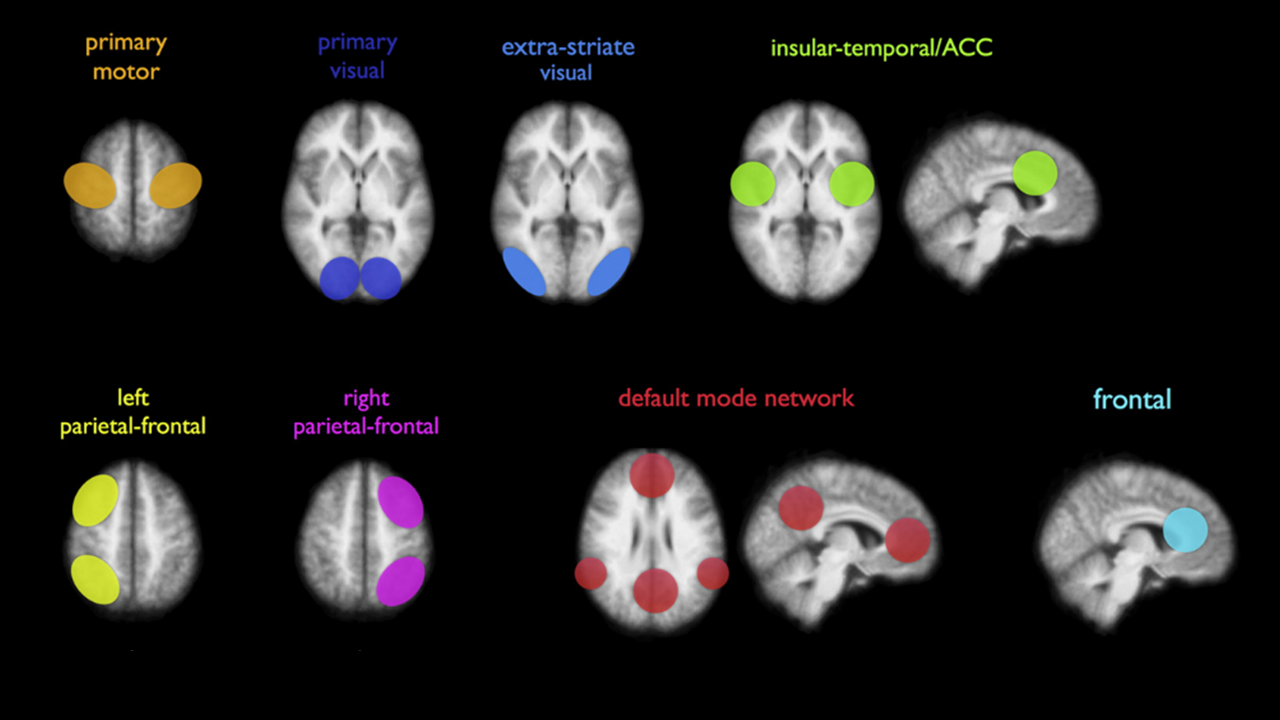
\includegraphics[height=3in]{images/ch1-ica.png}
    \caption[Examples of canonical resting-state networks.]{Examples of a few canonical resting-state networks observed in multiple studies with multiple methodologies from 1995 to 2010 \citep{Biswal1995, Beckmann2005, DeLuca2006,VandenHeuvel2009}. Subsequent parcellations such as that of Yeo and colleagues in 2011 formalized the notion that all brain areas are associated with an intrinsic network \citep{Yeo2011}. Figure adapted from \citep{VandenHeuvel2010}.}
    \label{fig:ch1-ica}
\end{figure}

A major advance in quantitative analysis of RSNs came with the introduction of graph theory techniques to the field. One of the major early findings was that the brain is organized in a complex but efficient ``small-world'' architecture. That is, a set of ``hub'' areas have disproportionate influence in connecting disparate brain areas. The concept has implications for cognitive models and neurology: for example, lesions on areas that are not densely connected showed less extended impairments than regions which are hub-like in RS-fMRI analyses \citep{Warren2014}. Even less severe disorders appear to have disrupted network architecture: researchers observed a reorganization of RSNs and decrease of modularity in individuals with depression \citep{Lord2012}. Thus network properties may be important for explaining individual differences in neuropsychiatric disorders or cognitive skill, such as comprehension.

In the graph model of the brain, the brain is modeled as a set of ``nodes'' connected by ``edges''. Typically, one of several approaches has been used to identify nodes: anatomical parcellations based on an atlas \citep{Supekar2008, Liu2008, Lynall2010}; individual voxels \citep{Fair2007}; functional ROIs from either a priori hypotheses or task-based activation \citep{VandenHeuvel2010}; or an algorithm that parcellates the brain independent of function or anatomy \citep{Goni2014}. Differences in these methods can affect the RSNs identified. At high resolutions (e.g. voxel-level correlations), there is a greater chance of spurious correlations causing noise in the data; at lower resolutions, the timeseries for a region may blend multiple functional regions, creating a composite that does not truly reflect any of the underlying areas. 

The edges connecting each node can be binary or weighted, in which case areas that are more highly correlated carry a greater connectivity value. The decision of how many and what type of edges to include is crucial because many of most interesting characteristics, including modularity and small-worldness, only emerge when the graph has been thresholded to a certain level of sparsity \citep{Moussa2012}. It is now common to sweep analyses across a number of edge-forming thresholds in order to ensure that arbitrary selection of edges is not unduly influencing analytical results.

\begin{figure}[t]
    \centering
    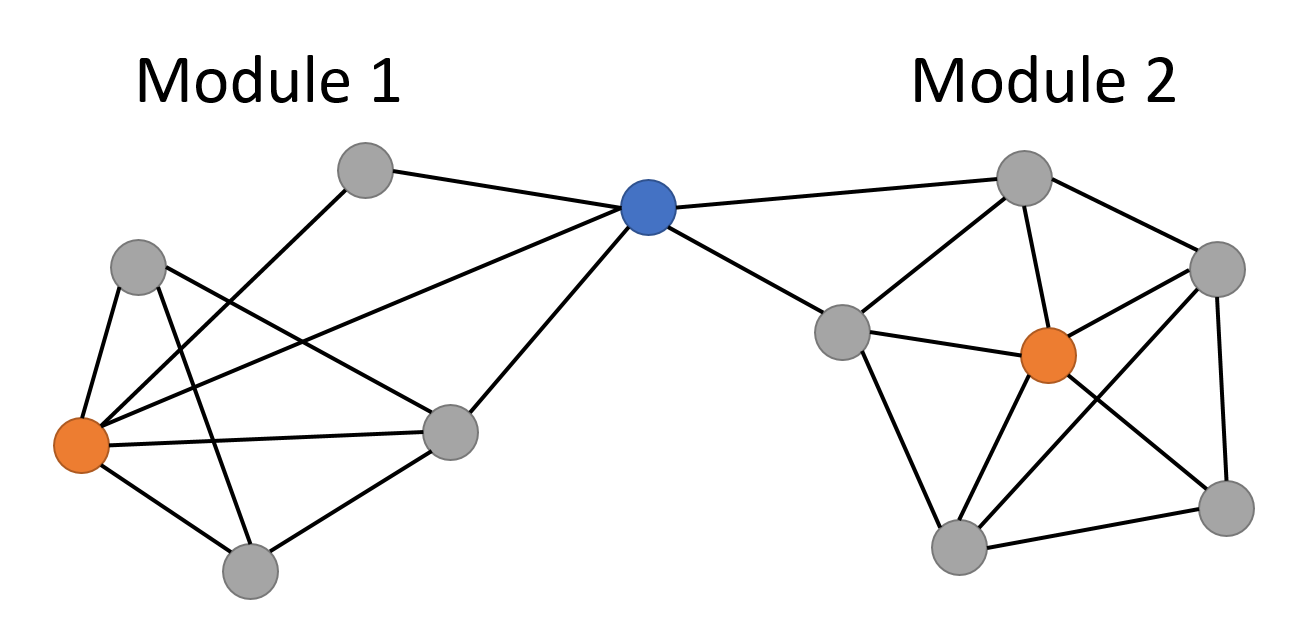
\includegraphics[height=3in]{ch1-graph-schema}
    \caption[Schematic for a network with two modules.]{Schematic for a network with two modules, or resting-state networks. A high proportion of within-module edges leads to high modularity; a large proportion of between-module edges leads to high participation coefficient. Figure credit to Godwin et al. \citep{Godwin2016}}
    \label{fig:ch1-graph-schema}
\end{figure}

Graph theory measures abound, and there is currently no consensus as to which measures are most appropriate in a general sense. In the following studies, we focus on three. \textit{Modularity} is the number of connections a single node has \citep{Sporns2013}. Nodes with higher degrees are thought to communicate with a greater number of nodes than others; networks with a higher average degree are thought to be more densely connected. \textit{Participation coefficient} is the degree to which a node participates in networks other than its primary one. The \textit{shortest path length}, or simply ``path length'', is the minimum number of edges that must be traversed to connect one node to any other. Small-world networks like the brain utilize ``hubs'' to maintain a relatively short path length from any one node to another. 

While hundreds of studies have been published utilizing graph theory, the neurobiological basis of these metrics is still under investigation. While these connections do appear to be plastic and mediated by experience, they are not necessarily caused by new synapses. Several studies using diffusion-weighted MRI (DW-MRI) suggest that functional connectivity represents more than simply direct synaptic connections. DW-MRI uses water movement to model the white matter tracts within the brain. At high resolutions, it provides a coarse approximation of the human connectome, i.e. the total connections in the human brain \citep{Sporns2005}. Honey et al. investigated whether functional connectivity can be predicted from structural connectivity and found that, while structurally connected areas are typically functionally connected as well, the inverse is not true \citep{Honey2009}. Areas that were closer together were also more highly functionally connected, possibly due to structural cortico-cortical projections. 


\section{The role of network architecture in reading}
While reading researchers in the past decade have begun to acknowledge the contributions of domain-general skills (e.g. attention, working memory, planning and organizing) to reading, it remains a secondary concern in much neuroimaging literature. (This is not the case for all language research but specifically reading.) To illustrate the widespread distribution of activity, we compared the meta-analytic activations maps from NeuroSynth with a popular resting-state network parcellation \citep{Bailey2018}. 

The results, shown in figure \ref{fig:ch1-yeo-to-neurosynth}, show that the visual and somatomotor-auditory RSNs consituted about one quarter of the NeuroSynth activations (17.5 and 8.2 percent, respectively), while attention networks combined to make up 37 percent. The fronto-parietal (19.3 percent) and default mode (17.8 percent) networks were were also highly represented. The limbic network was the only RSN which did not meaningfully overlap with the reading network. The visual makes clear what is well-known: reading areas are well-distributed across different networks and load highly onto attention and executive networks. Several important reading areas, including the inferior frontal gyrus and temporo-parietal junction, sit at points where multiple networks converge, i.e. likely hub areas.

\begin{figure}[t]
\centering
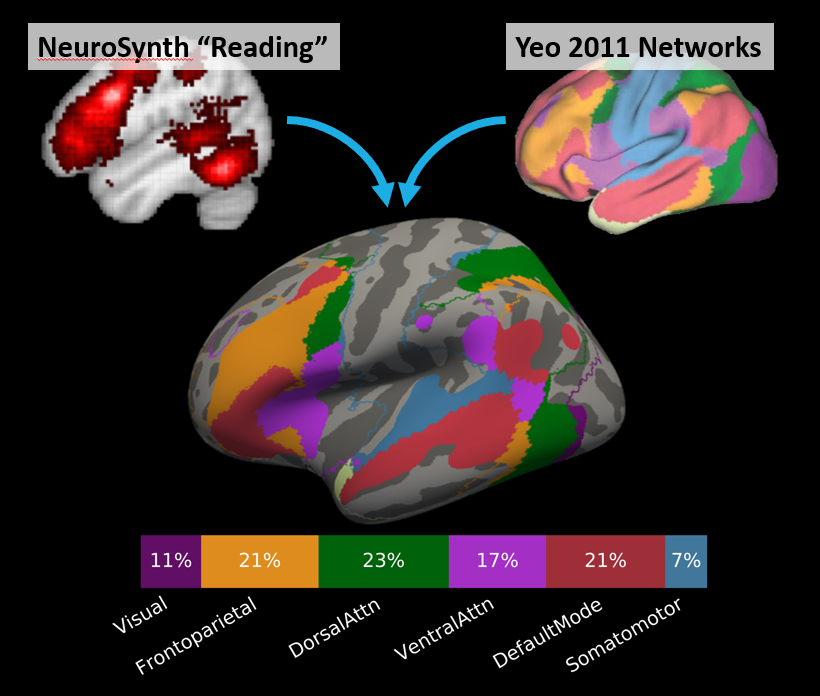
\includegraphics[height=3in]{images/ch1-yeo-to-neurosynth.png}
    \caption[Reading areas are distributed across many resting-state networks.]{Reading areas are distributed across many resting-state networks. On the left is the volumetric breakdown of the ``reading'' network, pulled from a NeuroSynth automated meta-analysis (forward-inference: $p < 0.01$, FDR-corrected) \citep{Yarkoni2011}, according to the 7-network cortical parcellation from Yeo and colleagues \citep{Yeo2011}.}
    \label{fig:ch1-yeo-to-neurosynth}
\end{figure}

In the next few sections, we survey possible functions of these RSNs and hub areas might play during reading and in dyslexia.  

\subsection{The visual word form area as part of the dorsal attention network} 
The visual word form area (VWFA) performs an important role in orthographic processing, namely processing lexical and sublexical stimuli. Activity in the VWFA is thought to be insensitive to letter size, font and other orthographic attributes \citep{Cohen2002}. However, its alleged specificity to language has been a source of controversy over the past decade, and some have argued that its importance in reading is directly linked to its membership in the dorsal attention network (DAN) \citep{Vogel2012a}, which supports the parsing of appropriate textual features and suppressing distracting information elsewhere \citep{Corbetta2002}. At issue in the debate is how general or specific visual attention deficits are in dyslexia \citep{Vogel2014}. Although decreased activation in the pVWFA to text relative to typically developing participants has been reported in several studies of dyslexia, these differences could be due to more generalizable visuo-spatial deficits  \citep{Richlan2009}. For example, fluent reading requires accurate and precise eye movements \citep{Rayner1978}, and a key node in the DAN is the ``frontal eye fields'' which help coordinate saccadic activity \citep{Connolly2002}. In fact, a number of studies report deficits in visual attention, rather word recognition, in children with RD \citep{Vidyasagar2010}.  Whatever the true cause, it is clear that the DAN provides critical support for reading, above and beyond simply processing stimuli.

\subsection{Attention networks drive and suppress sensory integration} 
Attention underlies skilled reading at all levels: it is critical for identifying only the salient words in a large block of text, for suppressing environmental distractions and for maintaining focus for extended periods of time. In a common framework for attention, the DAN and ventral attention network (VAN) play collaborative roles for guiding activity. (A third ``salience'' network is sometimes differentiated from the VAN.) Simplistically, the DAN exerts top-down control of sensory processes to keep a person on task, while the VAN acts as a ``circuit breaker'' to help reorient the person by detecting salient or unexpected stimuli \citep{Corbetta2002, Vossel2014}. This relationship may be impaired in individuals with dyslexia that have ``sluggish attention shifting'' between visual and auditory modalities \citep{Harrar2014}. Slow or inadequately rapid attention-shifting could undermine fluent reading by causing temporal-spatial misalignment in processing, e.g. letter sequence and arrangement \citep{Lallier2009}. This deficit in attentional shifting is argued to further characterize dyslexic readers' rapid temporal and low spatial frequency processing \citep{Witton1998}, and asynchronicity within this system is argued to be characteristic of dyslexia \citep{Lallier2009}. Online interaction between the DAN and VAN during reading may thus index some of the attentional switching problems that are apparent in dyslexia. 

\subsection{Executive networks coordinate other cognitive processes} 
Executive functions play an important role in predicting reading outcomes, especially when considering comprehension \citep{Cutting2009a}. Although the variety of cognitive processes that fall under EF construct do not map cleanly onto a single brain region or network, they are closely associated with the ``central executive'' system. This in turn is mapped on to the fronto-parietal and cingulo-opercular network (FPN and CON) \citep{Fedorenko2014a, Cocchi2013}. Unlike many other RSNs, the FPN has components which are not neighboring, spanning portions of the frontal and parietal lobes \citep{Yeo2011}. Interestingly, the FPN has recently been hypothesized to act as a neural mediator of other brain systems \citep{Menon2010, Cole2014} by using wide-spread cortical connections to facilitate efficient processing of other networks, and in particular assist when areas are not functioning adequately. According to this coordinator model of the FPN, greater symptoms of dyslexia may correspond with reduced functional and structural integrity of the FPN. And indeed there is some support: researchers have found de-activation and de-coupling of the FPN during a word rhyme judgment task in double deficit dyslexics \citep{Norton2014}, and in one of the only functional connectomics paper on young readers with dyslexia, another group found that whole-brain connectivity during a word/non-word rhyming task, and found that individuals with dyslexia showed de-coupling of frontoparietal areas \citep{Finn2014}. 

\subsection{Executive networks may support intervention response}
In addition to coordinating other RSNs, the FPN may play a role in supporting systems \citep{Cole2014}. In the first reading study to examine functional interactions across networks, Aboud et al. found that, prior to intervention, readers who were responsive to the intervention mediated reading network connectivity via a key node in the FPN, the dorsolateral prefrontal cortex \citep{Aboud2018}.  Other studies have had similar findings, with a less coherent network perspecitve. In one study, readers with and without dyslexia underwent a reading intervention. After intervention, readers with dyslexia had increased connectivity between a visual component and bilateral regions in the FPN (notably, as in many studies on reading, the latter component was not identified as an FPN component, but instead discussed as a language network) \citep{HorowitzKraus2015}. Another group examined resting state connectivity in dyslexic readers with variable remediation status, and found that children with a historical diagnosis of dyslexia had persistent de-coupling of frontoparietal areas compared to typical readers, regardless of remediation status \citep{Koyama2013}. Taken together, these findings support the hypothesis that executive areas in the FPN might act to facilitate the functional integrity of other systems necessary for reading.

\subsection{Default mode network engagement and disengagement} 
The default mode network (DMN) spans the medial prefrontal cortex, bilateral inferior parietal lobules, and posterior cingulate cortex \citep{Raichle2001}. Since its original discovery, the DMN has since been found to support a wide range of cognitive processes often classified under internal mentation \citep{Buckner2008}, including theory of mind, narrative processing, and autobiographical recall \citep{AbdulSabur2014}. The DMN has a large amount of overlap with traditional language areas, including comprehension-related regions such as the angular gyrus and anterior temporal pole. However, the DMN also has antagonistic relationship with ``task-positive'' attention networks such as the FPN, where the activation of one network necessarily comes at the suppression of the other, and this relationship appears to be important for performance on a variety of cognitive processes \citep{Fox2005, Keller2015}. Consequently, appropriate FPN involvement may be best achieved by suppression of the DMN. Several studies point to over-involvement of the DMN in readers with dyslexia, including higher internal correlations of the DMN during reading \citep{Finn2014} and greater correlations between the DMN and reading areas during reading and at rest \citep{Schurz2014}. Given that activity in both the FPN and DMN are critical for reading comprehension, understanding the dynamics of this relationship could be illuminating.

\subsection{Hub areas show abnnormalities in dyslexia}
A particularly intriguing hypothesis is that dyslexia may be associated with differences in the brain's hub network, those areas that are responsible for integrating information across many different RSNs. To determine whether there was any pattern related to network architecture in dyslexia-related areas, we gathered all clusters from three meta-analyses comparing fMRI activation for individuals with dyslexia to typical readers \citep{Maisog2008, Richlan2009, Paulesu2014}. All areas that showed atypical activation in dyslexia (either greater or less activity) were included.

\begin{figure}[t]
\centering
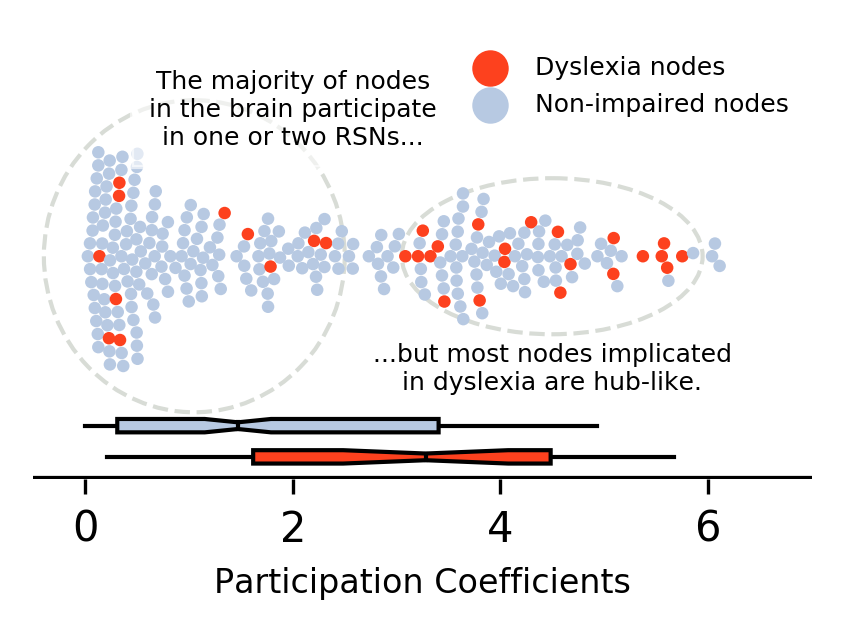
\includegraphics[height=3in]{images/ch1-dyslexia-hubs.png}
    \caption[Dyslexia disproportionately impacts hub areas.]{Dyslexia disproportionately impacts hub areas. Among the brain areas examined in Power and colleagues (2013), nodes implicated in dyslexia have higher participation coefficients (32 nodes) compared to the rest of the brain (232 nodes).}
\label{fig:ch1-dyslexia-hubs}
\end{figure}

To get measures of hubness across the brain, we used data from a connectomics study \citep{Power2013}. That study reports the \textit{participation coefficient} for each of the 264 nodes previously described. As discussed, the participation coefficient reflects the diversity of a node's connectivity to different RSNs, where a higher value indicates that the node is correlated with many different RSNs. Activations from the dyslexia meta-analyses were then mapped to the geometrically closest node from this dataset, resulting in a small set of dyslexia-related nodes and a larger, unaffected set.

The distribution of participation coefficients across the 264 nodes was non-normal, with a large group of areas having low participation coefficients (i.e. affiliated with few RSNs) and a smaller hub-like group. Figure \ref{fig:ch1-dyslexia-hubs} shows the node-by-node distribution of participation coefficients for the entire set. The results were unambiguous: dyslexia affects brain areas with higher participation coefficients than would otherwise be expected ($p$ \textless $0.001$) -- further evidence that a network architecture perspective on reading is likely to yield new insights. 

The finding that hubs areas are key in dyslexia are not surprising: dyslexia has often been thought to be a disorder of combining information across different functional systems, and in the context of connectomics, hub areas play a privileged role in mediating information flow between RSN’s. For example, the posterior temporal sulcus connects visual and auditory networks by binding letters to sounds \citep{Blau2010, VanAtteveldt2009} and the inferior frontal gyrus has many different subdivisions supporting language parsing and manipulation \citep{Hagoort2005}. However, casting dyslexia dysfunction into a connectomics perspective opens up new hypotheses and research avenues. For example, the brain areas of interest and neuroimaging metrics can be unified across other developmental disorders, including ADHD, specific language impairment and autism \citep{Stam2014}. Another benefit is that it opens up many more avenues for investigating dyslexia using functional and diffusion MRI, which can be performed in younger children and without administering a cognitive task. 


\section{Influence of development on network connectivity}

Children are taught to decode words between the ages of four and nine. This is a time of major developmental changes in the brain, with extensive synaptic pruning and myelination of white matter tracts \citep{Wandell2013}. The brain areas responsible for fast and efficient word decoding may become specialized through a process of \textit{interactive specialization}, in which intrinsic developmental processes and experience collaborate to form the mature, skilled reading system \citep{Johnson2011, Klingberg2014}. The theory is an extension of the Hebbian maxim that ``neurons that fire together, wire together'', with the brain being considerably more plastic during this developmental period than it is later in life \citep{Hebb1949}.

\begin{figure}[t]
    \centering
    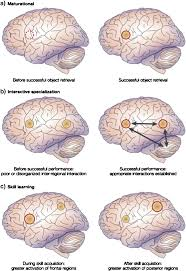
\includegraphics[width=4in]{images/ch1-interactive-specialization.jpg}
        \caption[Interactive specialization explains changes in activity.]{Interactive specialization posits that repeated co-activation of distant brain areas will create a network of regions important for performance of a given task. Figure credit to \citep{Gaffrey2013}.}
    \label{fig:ch1-interactive-specialization}
\end{figure}

Interactive specialization accommodates the observations that learning to read creates changes to connectivity that persist even at rest. In a series of studies, Maki Koyama found that individual connections between reading-related nodes was indicative of reading perofrmance improvement. They first found that many reading-related nodes had overlapping connectivity with the left inferior frontal gyrus and left middle temporal gyrus, both nodes that are important for skilled language use \citep{Koyama2010}. A follow-up study comparing IQ-matched children and adults found similar patterns: better readers in both groups showed increased connectivity between the inferior frontal gyrus and the middle and superior temporal gyri, as well as between the precentral gyrus and motor areas \citep{Koyama2011}. In adults, positive correlations were found between reading ability and connectivity between the visual word form area and phonological processing areas; in children, however, this correlation was weaker and negative, suggesting that the visual word form area becomes more integrated with experience as well as skill. Reading intervention also exerts an effect on connectivity patterns. Dyslexic adolescents who received reading remediation had higher correlations between the visual word form area and the right middle occipital gyrus than did control participants \citep{Koyama2013}. Connectivity values also correlated with spelling and single-word reading scores.

Despite the changes in connectivity between areas, reading-related regions such as the fusiform gyrus, angular gyrus and inferior frontal gyrus, do not create one distinct RSN, but are members of separate, more primary RSNs \citep{Vogel2013}. These RSNs exhibit increasing functional correlation across the lifespan \citep{Kesler2013, Uddin2010}. Their properties, including density of connections, along with their locations and changes with development are a major area of interest, but their study is difficult due to differences in motion across the populations \cite{Power2013}. Nevertheless, the general understanding is that RSNs in children are more greatly constrained by proximity than in adults but are nonetheless functionally organized. Visual system regions, for example, form their own community, as do auditory regions and executive control regions \citep{Seeley2007}. This small-world architecture appears to reach peak efficiency in young adulthood, with younger children exhibiting fewer long-range RSNs and older adults showing a decrease in modularity, especially in higher-order RSNs like the DMN \citep{Cao2016}. However, the relationships between development, expertise and network architecture have not yet been disentangled, and it is our hope that the current manuscript will spur further investigations into these issues. 

According to the view of interactive specialization, an integrative ability like reading comprehension would induce a transient, highly connected brain state. Repeatedly activating this network over time would result in the common pathways becoming more tightly connected. Individuals who can more easily access these widespread resources, i.e. who have more integrated connectomes, may be more likely to read well; older readers, too, would be expected to be more fine-tuned for comprehension. And because comprehension is a shared process between different regions, this network model may be even more telling than localized measures of brain function and activity. 


\section{Outstanding questions}

We have established that the network model of cognition has particular bearing in models of reading, and that graph theory methods provide a summary framework with which to investigate the interactions between processes. Furthermore, development of cognitive skills is facilitated by the interactions between regions, rather than solely by themselves - but the study of these processes have not been investigated extensively. These higher level processes are important for longer forms of reading -- passage reading, for example, which is more common in older readers. Although disentangling the contributions from other skills (working memory, attention, planning/organization) during reading is difficult for behavioral research \citep{Cain2006}, it is a question that is well-suited to neuroimaging studies. 

In this dissertation, we present four studies that investigate network properties as they relate to reading comprehension and reading success. The common thread is that reading requires the integration of many different brain networks (even moreso than listening) and that better readers are more able to meet these demands, even from a young age.

\begin{itemize}

    \item \textit{Study 1} investigates individual differences in ``intrinsic'' network architecture and its relationship to reading skill using resting-state fMRI dataset from older children (ages 9 to 11). We establish a set of methods for analyzing variability in connectomes, and address the question of whether some individuals are better equipped to handle the additional complexity of reading. 

    \item \textit{Study 2} describes how network architecture changes \textit{during} reading. We examine changes within and between RSNs and attempt to localize these differences to specific RSNs, such as the visual, dorsal attention and default mode networks. We also elaborate on the results of Study 1, testing whether the relationship between network architecture and reading skill changes in the task-evoked connectome. 

    \item \textit{Study 3} moves beyond looking only at reading-evoked activity by first comparing reading to listening comprehension, then to several other activities. The key questions this study addresses are whether greater variability between task-evoked networks is a beneficial attribute, and whether any particular RSNs (such as the fronto-parietal network) are more responsible for the reconfiguration of the whole-brain network.

    \item \textit{Study 4} follows up on the modality results by analyzing network topology during reading comprehension across development. These analyses serve as a replication and extension of each of the previous studies: we test whether the relationship between reading and network architecture changes in more mature individuals and how task-evoked activity differs along the lifespan. While there is strong evidence that learning to decode creates persistent changes to the neural systems utilized in language \citep{Schlaggar2007}, there have been no studies investigating the trajectory of brain modularity and its changes to reading over time.

\end{itemize}

Overall, these studies will use reading-related brain activity and behavior as a model for understanding how individual differences in network architecture form a basis for individual differences in cognitive processing. We combine inferences from several different methodological approaches, including resting-state network analysis, task-based activation analyses, and the combination of the two. Through this systematic approach to describing these samples, we strive to make a meaningful contribution to our understanding brain modularity and its relationship to cognition.